% Shared preamble for the English summaries in this repository.
\documentclass[11pt,a4paper]{article}
\usepackage[margin=2.2cm]{geometry}
\usepackage[T1]{fontenc}
\usepackage[utf8]{inputenc}
\usepackage{lmodern}
\usepackage{amsmath,amssymb}
\usepackage{graphicx}
\usepackage{booktabs}
\usepackage{enumitem}
\usepackage[hidelinks]{hyperref}
\setlist{itemsep=2pt,topsep=4pt}
\setlength{\parindent}{0pt}
\setlength{\parskip}{5pt}
\graphicspath{{figures/}}
\newcommand{\summaryheader}[3]{%
  \begin{center}
    {\Large\bfseries #2}\\[3pt]
    {\large #1}\\[3pt]
    {\small Arshia Goshtasbi \textbullet{} MSc Electrical Engineering (Control), Iran University of Science and Technology \textbullet{} #3}
  \end{center}
  \vspace{2pt}\hrule\vspace{8pt}\par}

\begin{document}
\summaryheader{Reinforcement Learning, HW6--HW8 and Comprehensive Exercise Q2}{Reinforcement Learning for Optimal Control}{Autumn 1403 (2024)}

Each problem below has an exact answer, so every learned controller is compared with it.

\section*{1. Discrete-time LQR (HW6)}
Plant $x_{k+1}=Ax_k+Bu_k$ with three states, $Q=I_3$, $R=1$, $u=-Kx$. From $K_0=0$ (the plant is stable):
\begin{itemize}
  \item \textbf{Policy iteration:} $(A-BK_j)^\top P_{j+1}(A-BK_j)-P_{j+1}+Q+K_j^\top RK_j=0$, then $K_{j+1}=(R+B^\top P_{j+1}B)^{-1}B^\top P_{j+1}A$.
  \item \textbf{Value iteration:} $P_{j+1}=(A-BK_j)^\top P_j(A-BK_j)+Q+K_j^\top RK_j$ with the same improvement step.
  \item \textbf{$\lambda$-policy iteration:} $P_{j+1}=(1-\lambda)A_j^\top P_jA_j+\lambda A_j^\top P_{j+1}A_j+K_j^\top RK_j+Q$, $A_j=A-BK_j$; $\lambda=1$ is PI and $\lambda=0$ is VI.
  \item \textbf{Model-free Q-learning:} $Q_K(x,u)=[x;u]^\top H[x;u]$ is fitted from measured transitions with $z_k^\top Hz_k-z_{k+1}^\top Hz_{k+1}=x_k^\top Qx_k+u_k^\top Ru_k$, and $K\leftarrow H_{uu}^{-1}H_{ux}$.
\end{itemize}
All reach the DARE gain $K^*=[-0.06432,\ -0.06989,\ 0.06668]$: PI in 5 iterations, $\lambda=0.9$ in 78, $\lambda=0.5$ in 318, VI in 605, Q-learning in 4 (from data only, error $6\times10^{-15}$).

\begin{center}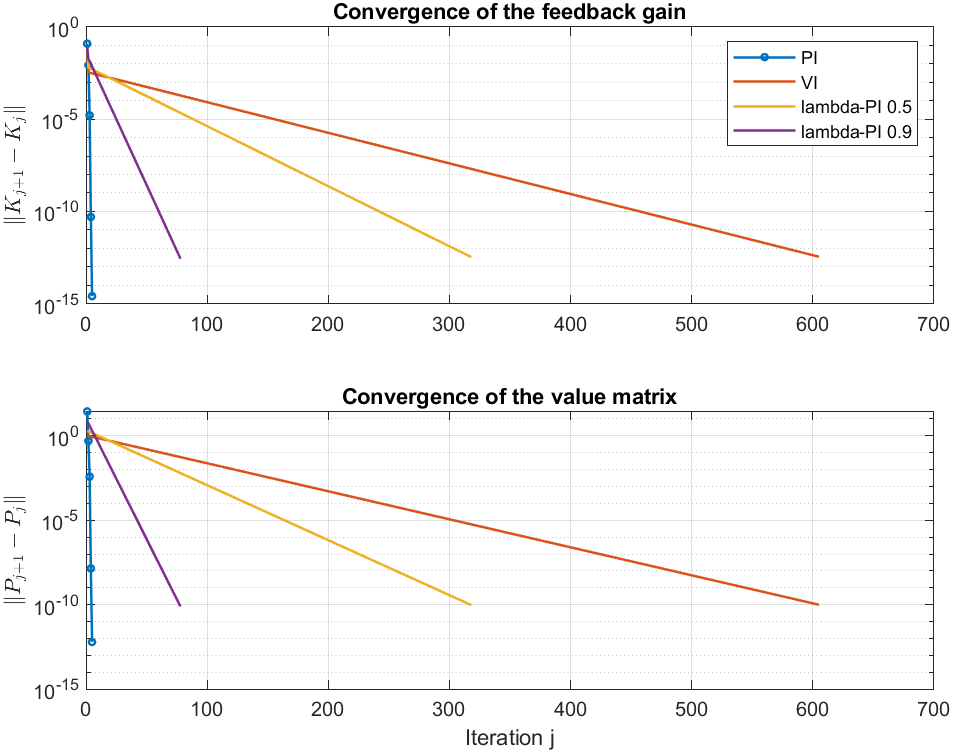
\includegraphics[width=0.62\textwidth]{dt_lqr_pi_vi.png}\end{center}

\section*{2. Integral RL and off-policy $H_\infty$ control (HW7)}
\textbf{IRL.} For $\dot x=Ax+Bu$ and $u=-K_jx$, $V_j=x^\top P_jx$ satisfies
$x(t)^\top P_jx(t)-x(t{+}T)^\top P_jx(t{+}T)=\int_t^{t+T}x^\top(Q+K_j^\top RK_j)x\,d\tau$. $P_j$ is fitted from measured states (no $A$), then $K_{j+1}=R^{-1}B^\top P_j$. It reached the CARE gain $[-0.13523,\ -0.15010,\ 0.43293]$ in 4 iterations.

\textbf{$H_\infty$ control} with disturbance $d$ and $\beta=5$: the reference is the game Riccati equation $A^\top P+PA+Q-PB_1R^{-1}B_1^\top P+\beta^{-2}PB_2B_2^\top P=0$. With data from an exploring behaviour policy and target policies $u_j=-K_{1j}x$, $d_j=K_{2j}x$,
\[
x^\top P_jx\Big|_t^{t+T}=\int_t^{t+T}\!\big[-x^\top(Q+K_{1j}^\top RK_{1j}-\beta^2K_{2j}^\top K_{2j})x+2(u+K_{1j}x)^\top RK_{1,j+1}x+2\beta^2(d-K_{2j}x)^\top K_{2,j+1}x\big]d\tau,
\]
which is linear in $(P_j,K_{1,j+1},K_{2,j+1})$ and needs no model. It matched the game Riccati solution in 3 iterations ($\|P-P^*\|=2\times10^{-5}$). For $w(t)=0.2e^{-0.2t}\cos t$ the measured attenuation ratio is 0.77, below $\beta=5$.

\begin{center}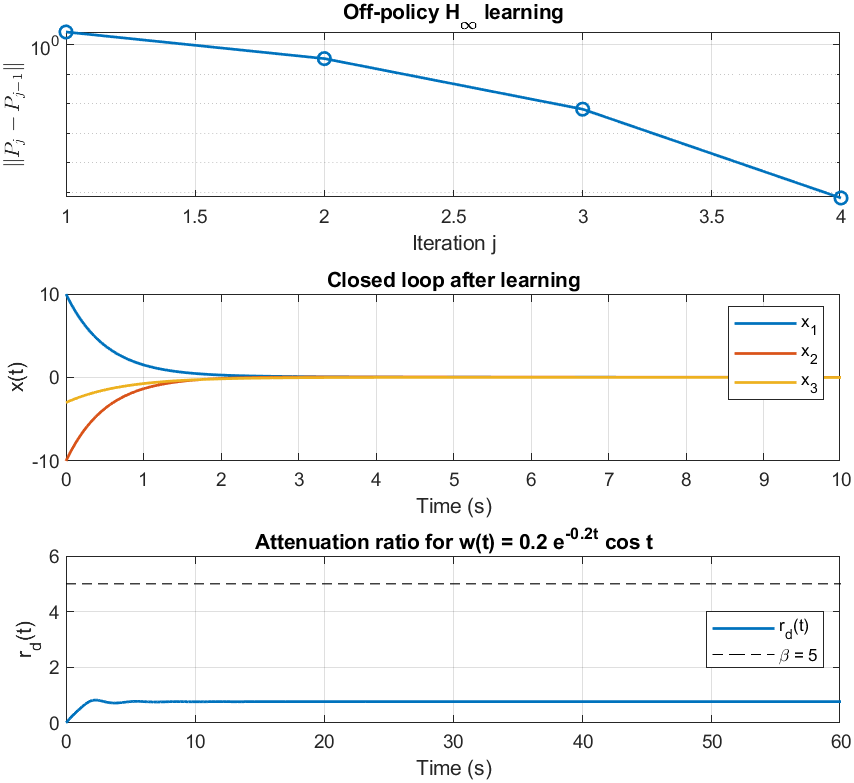
\includegraphics[width=0.62\textwidth]{ct_offpolicy_hinf.png}\end{center}

\section*{3. Actor-critic for a nonlinear system (HW8)}
For $\dot x_1=x_2$, $\dot x_2=-x_1(\tfrac{\pi}{2}+\arctan 5x_1)-\tfrac{5x_1^2}{2(1+25x_1^2)}+4x_2+3u$ with $Q=\mathrm{diag}(0,1)$, $R=1$, the optimum is $V^*=x_1^2(\tfrac{\pi}{2}+\arctan5x_1)+x_2^2$, $u^*=-3x_2$. With critic basis $\phi=[x_1,\,x_2,\,x_1x_2,\,x_1^2,\,x_2^2,\,x_1^2\arctan5x_1,\,x_1^3]$ and actor $u=W_ax_2$, the continuous-time actor-critic alternates a critic fit of $W_c^\top(\phi(x(t))-\phi(x(t{+}T)))=\int r\,d\tau$ and an actor fit to $-\tfrac12R^{-1}g^\top\nabla\phi^\top W_c$. Starting from $W_a=-2$ it reached $W_c=[0,0,0,\pi/2,1,1,0]$ to four decimals and $W_a=-3.00003$ in 4 iterations.

\begin{center}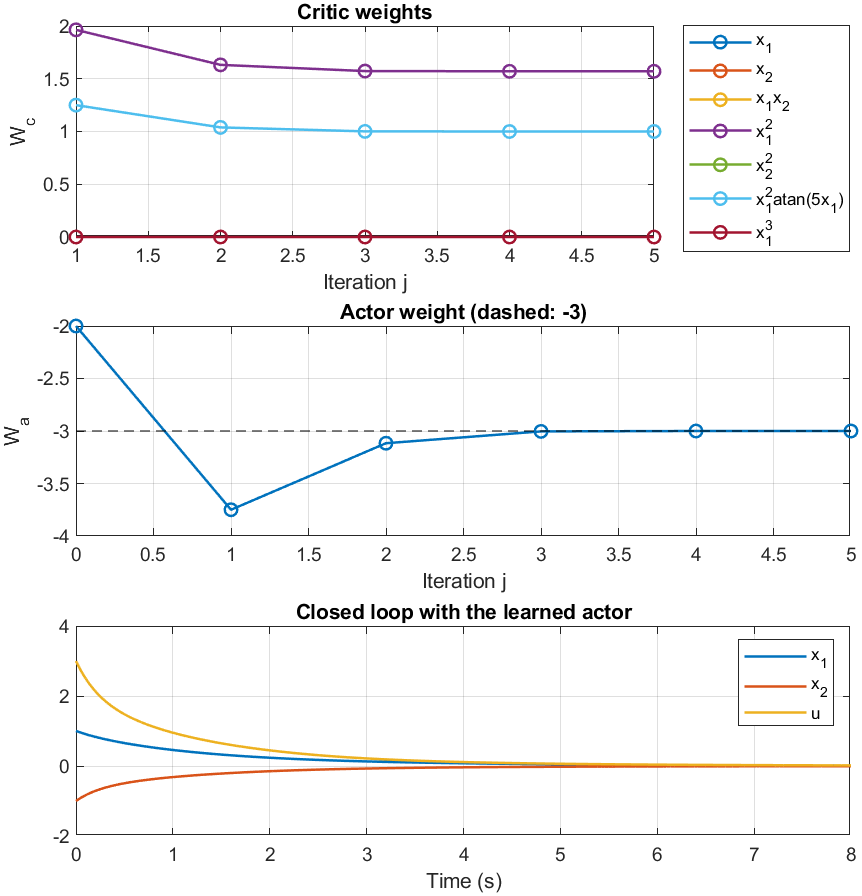
\includegraphics[width=0.62\textwidth]{ct_actor_critic.png}\end{center}

\section*{4. On-/off-policy IRL and tracking (Comprehensive Q2)}
For the unstable plant $A=\begin{bmatrix}0.5&1.5\\2&-2\end{bmatrix}$, $B=[1;4]$, both IRL variants reach the CARE gain $[1.6180,\ 0.9001]$. Off-policy IRL (one batch of behaviour data, no model) reaches $\|P-P^*\|=6\times10^{-7}$; on-policy IRL stalls near $10^{-4}$ because its probing noise enters the Bellman equation as a bias, which the off-policy form avoids. For tracking $x_d=[\sin t;\cos t]$ I used the augmented state $X=[e;x_d]$ and the discounted Bellman equation $X(t)^\top PX(t)=\int_t^{t+T}e^{-\gamma(\tau-t)}r\,d\tau+e^{-\gamma T}X(t{+}T)^\top PX(t{+}T)$. The learned gains match the discounted ARE to about $10^{-3}$ for $\gamma=0.4$ and $0.9$; the tracking error stays near 0.7 because the discounted problem with $R=3$ does not force it to zero.

\begin{center}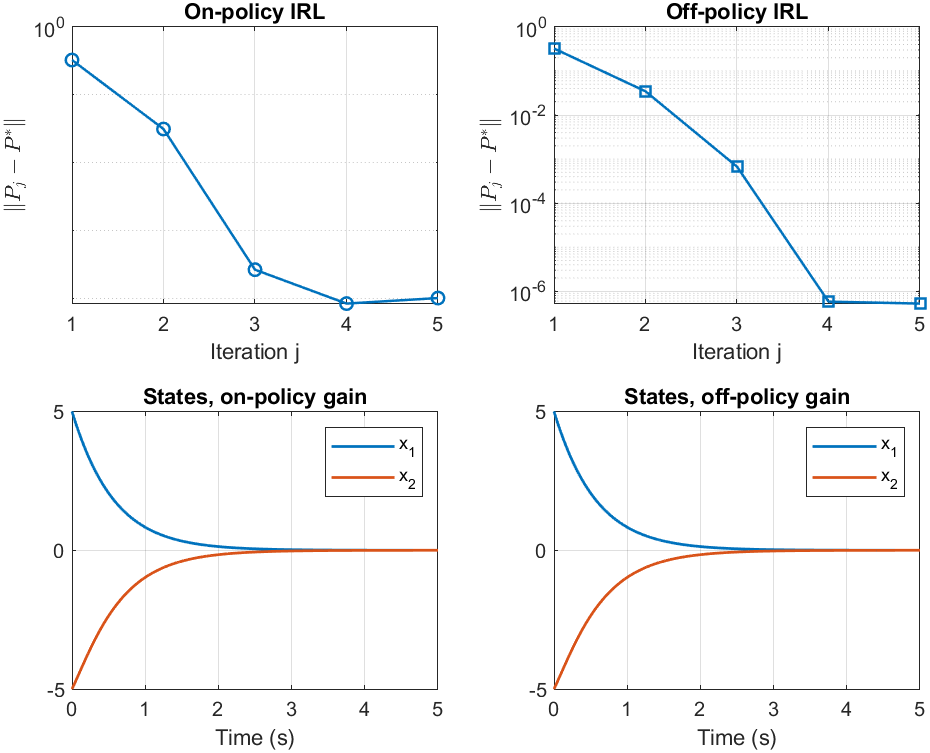
\includegraphics[width=0.62\textwidth]{irl_on_off_policy.png}\end{center}
\end{document}
